\section{Introduction}
	Enzymes can catalyze chemical reactions by lowering the energy barrier which is needed to be crossed over during the reaction. A general enzyme-catalysed reaction is described as the following form,
	\begin{equation}
	\ce{E + S <=>[$k_1$][$k_2$] ES ->[$k_3$] E + P},
	\label{eq:chemical}
	\end{equation}
	which involves an enzyme E, a substrate S and a product P. In this reaction, E and S firstly bind together to form a complex ES, and ES then releases the product P. Here $k_1$, $k_2$ and $k_3$ are the corresponding first-order rate constants. If denoting the concentrations of each component as $C_E$, $C_S$, $C_{ES}$ and $C_P$, the dynamics of this reaction is formulated by the following master equation.
	\begin{equation}
	\dv{}{t}\begin{pmatrix*}[l] C_E \\ C_{ES} \\ C_S \\ C_P \end{pmatrix*} = 
		\begin{pmatrix*}[r]
			-1 &  1 &  1 \\
			 1 & -1 & -1 \\
			-1 &  1 &  0 \\
			 0 &  0 &  1 
		\end{pmatrix*}
		\begin{pmatrix} v_1 \\ v_2 \\ v_3\end{pmatrix},
	\label{eq: original_equation}
	\end{equation} 
	where the matrix is called stoichiometric coefficient matrix and the entities of its three columns are corresponding to stoichiometric coefficients of the three reactions. And $v_1$, $v_2$, $v_3$ denote the reaction speed, i.e.
	\begin{equation}
		\begin{aligned}
			v_1 &= k_1 C_S C_E \\
			v_2 &= k_2 C_{ES} \\
			v_3 &= k_3 C_{ES} \\
		\end{aligned}.
	\end{equation}

	In a typical enzyme-catalysed reaction, one may assume that $C_S$, $C_P$ are much higher than $C_E$ and $C_ES$, which results in the fact that $C_S$ are $C_P$ are approximately constants during a long-run. Thus the states of enzyme E (either as empyt E or as the complex ES) are considered as the major factor. This alows us to reduce the model by the following steps. First, omit the two rows of $C_S$ and $C_P$ in equation \eqref{eq: original_equation}. Next, divide $C_0 = C_E + C_{ES}$ on both sides of equation \eqref{eq: original_equation}, and further define the pseudo-first order rate constant $\widetilde{k_1}=k_1C_S$. Then the original equation \eqref{eq: original_equation} can be reduced to
	\begin{equation}
	\dv{}{t}\begin{pmatrix*}[l] p_E \\ p_{ES} \end{pmatrix*} = 
		\begin{pmatrix*}[r]
			-1 &  1 &  1 \\
			 1 & -1 & -1 \\
		\end{pmatrix*}
		\begin{pmatrix*}[l] \widetilde{k_1}p_E \\ k_2p_{ES} \\ k_3p_{ES}\end{pmatrix*},
	\end{equation}
	or
	\begin{equation}
	\dv{}{t}\begin{pmatrix*}[l] p_E \\ p_{ES} \end{pmatrix*} = 
		\begin{pmatrix*}[r]
			-\widetilde{k_1} &  k_2+k_3 \\
			 \widetilde{k_1} & -k_2-k_3 \\
		\end{pmatrix*}
		\begin{pmatrix*}[l] p_E \\ p_{ES} \end{pmatrix*}.
	\label{eq: master_eq}
	\end{equation}
	Here the $p_i=C_i/C_0,\  i=\text{E}, \text{ES}$ is the probability that the enzyme is at state E or ES. This reduced dynamic system can be shown in figure \ref{img:dynamics}.

	\begin{wrapfigure}{l}{5.5cm}
		\centering
		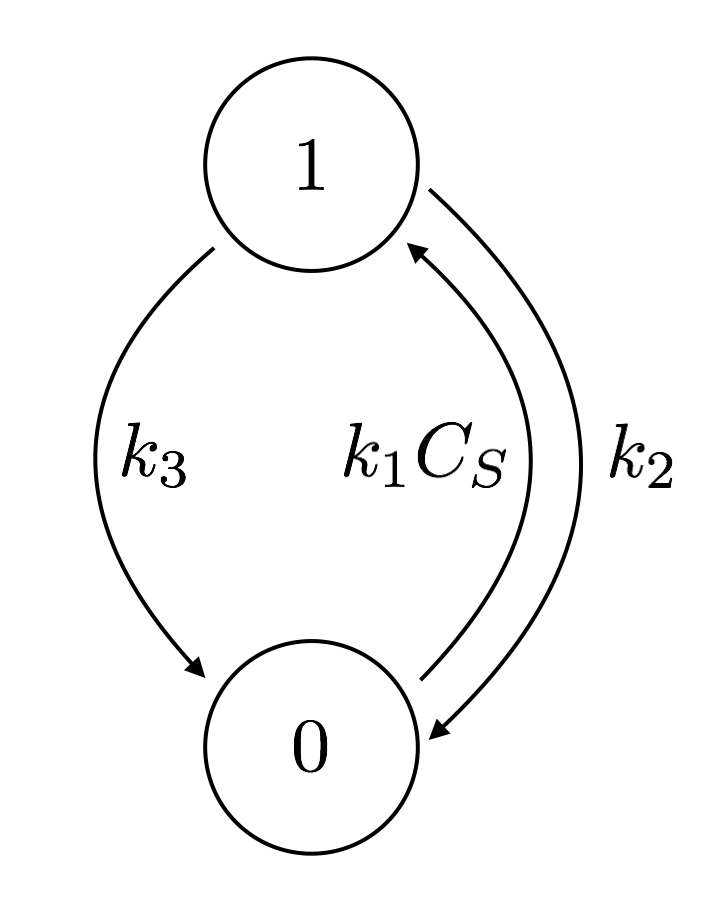
\includegraphics[scale=0.3]{img/dynamic_graph.png}
		\caption{dynamic graph of the system. state $0=$ E and $1=$ ES}
		\label{img:dynamics}
	\end{wrapfigure}

	Next we consider the situation when the system reaches a steady state, i.e. the l.h.s of equation \eqref{eq: master_eq} is zero. Notice that the normalization condition 
	\begin{equation}
		p_E + p_{ES} = 1
	\end{equation}
	should also be satisfied. So now we have three equations for only two variables, which means there is one redundant equation. To form a soluable linear system, we simply cancle the second row in equation \eqref{eq: master_eq}, then add the normalization condition into it. Finally the equation for the steady state becomes
	\begin{equation}
		\begin{pmatrix*}
			-\widetilde{k_1} &  k_2+k_3 \\
						1	 &  1 
		\end{pmatrix*}
		\begin{pmatrix*}[l] p_E \\ p_{ES} \end{pmatrix*} = 
		\begin{pmatrix*}[l] 0 \\ 1 \end{pmatrix*}	
		\label{eq: steady_state_eq}
	\end{equation}

	To understand the kinetics of the steady state, we can simply solve the equation \eqref{eq: steady_state_eq}, or use Gillespie Monte Carlo algorithm. These two methods will be discussed in the next section.

\section{Methods}
	\subsection{Analytic Solution}
		One straightforward method to solve the steady state equation \eqref{eq: steady_state_eq} analytically is Cramer's rule. The solution in this case simply is 
		\begin{equation}
			\begin{aligned}
				p_E &= \frac{k_2+k_3}{\widetilde{k_1}+k_2+k_3}\\
				p_{ES} &= \frac{\widetilde{k_1}}{\widetilde{k_1}+k_2+k_3}.
			\end{aligned}
			\label{eq:state_prob}
		\end{equation}

		Alternatiely, the solution can be written out by diagram method \cite{hill2004}. To apply this method, one need firstly construct partial graphs, which are undirected graphs containing the maximum number of edges without forming any cycles. In this case, there are two of them, as shown in figure \ref{img:partial_graphs}. Then, by adding arrows into the partial graphs, directed graphs are formed. There are three of them in this case, as shown in figure \ref{img:tree_graphs}.

		\begin{figure}[H]
		\centering
		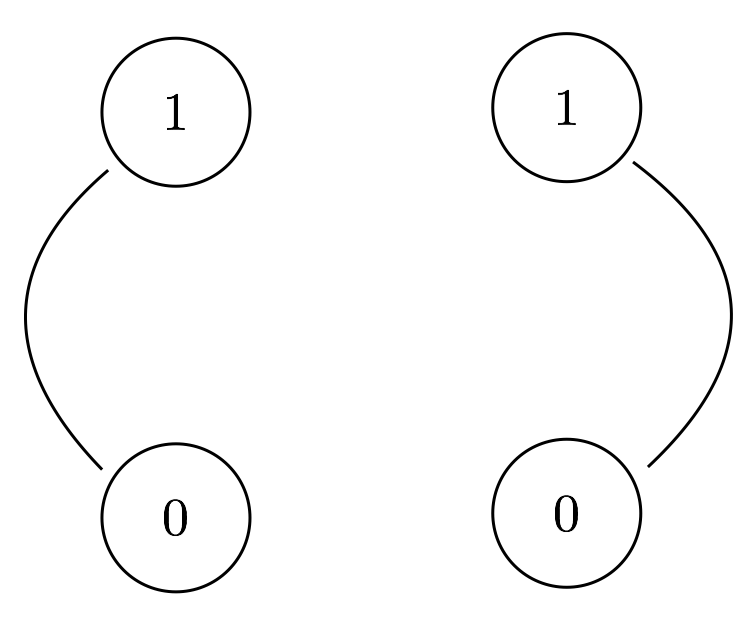
\includegraphics[scale=0.3]{img/partial_graph.png}
		\caption{partial graphs of figure \ref{img:dynamics}}
		\label{img:partial_graphs}
		\end{figure}
		\begin{figure}[H]
		\centering
		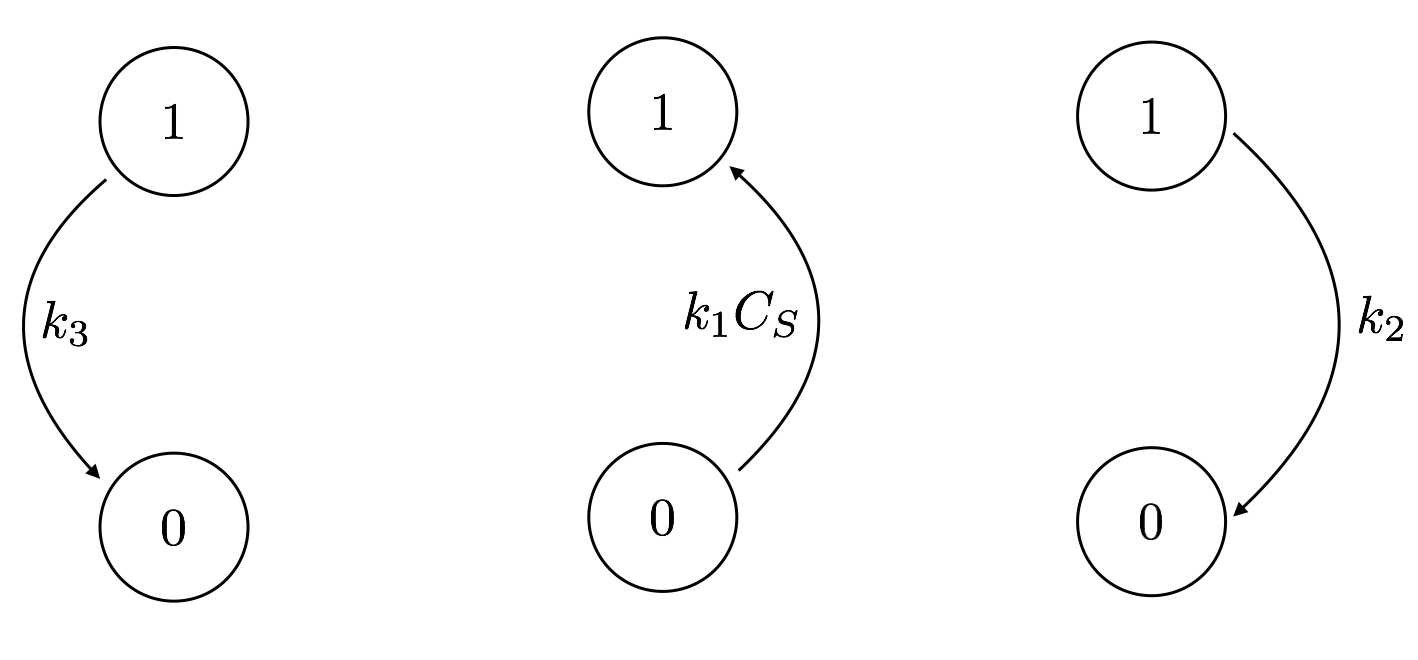
\includegraphics[scale=0.3]{img/tree_graph.png}
		\caption{directed graphs following the partial graphs}
		\label{img:tree_graphs}
		\end{figure}
		\noindent Each graph in figure \ref{img:tree_graphs} is corresponding to a rate constant (or a product of rate constants in a general case), Then the state probabilities are
		\begin{equation}
			p_i = \frac{ \text{sum of directed graphs with state $i$ being pointed to} }{ \text{sum of all directed graphs} }.
		\end{equation}
		By calculating so, equation \eqref{eq:state_prob} will be recovered exactly.

		A major concern here would be the product rate of this reaction regime. The product rate in this case can be described by the probability flux from state $1$ to $0$ through the left path with the rate constant $k_3$,
		\begin{equation}
			\begin{aligned}
				J_{1\rightarrow0}^{k_3} = k_3 p_{ES} 
					= \frac{k_3 \widetilde{k_1}}{\widetilde{k_1}+k_2+k_3} . 
			\end{aligned}
		\end{equation}
		$J_{1\rightarrow0}^{k_3}$ means, for one enzyme molecule E, the average number of reactions with rate constant $k_3$ which take place per unit time, i.e. the product rate with one enzyme in the system. If we consider the total product rate $v_P$ in a solution, the initial concentration of the enzymes should be multiplied. Then the Michaelis Menten equation \cite{michaelis1913} is recovered.
		\begin{equation}
				v_P = C_0 J_{1\rightarrow0}^{k_3} = \frac{v_{\text{max}} C_S}{C_S + K_M},
				\label{eq:MM}
		\end{equation}
		where $v_{\text{max}}=k_3C_0$ denotes the maximum product rate and $K_M=k_2+k_3/k_1$ is the Michaelis constant. This analytic result will be compared with Gillespie Monte Carlo simulation result in the last section.

	\subsection{Gillespie Monte Carlo Algorithm}

		The core idea of Gillespie Monte Carlo algorithm \cite{gillespie1976,gillespie1977} is to characterize the kinetic properties of the system by \textit{reaction probability density} $\rho(\mu,\tau)$, where $\mu$ denotes all possible transitions with respect to current state, and $\tau$ is a positive quantity called transition time. In this regime, $\rho(\mu,\tau)\diff \tau$ means the probability that the very first reaction that takes place in the infinitesimal interval $(t+\tau, t+\tau + \diff \tau]$ is the $\mu$th reaction. That is, more explicitly, the probability that no reaction takes place from current time $t$ until $t+\tau$, while the $\mu$th reaction then takes place in the next $\diff \tau$ time, as illustrated in figure \ref{img:reaction_prob}.

		\begin{wrapfigure}{r}{5.5cm}
		\centering
		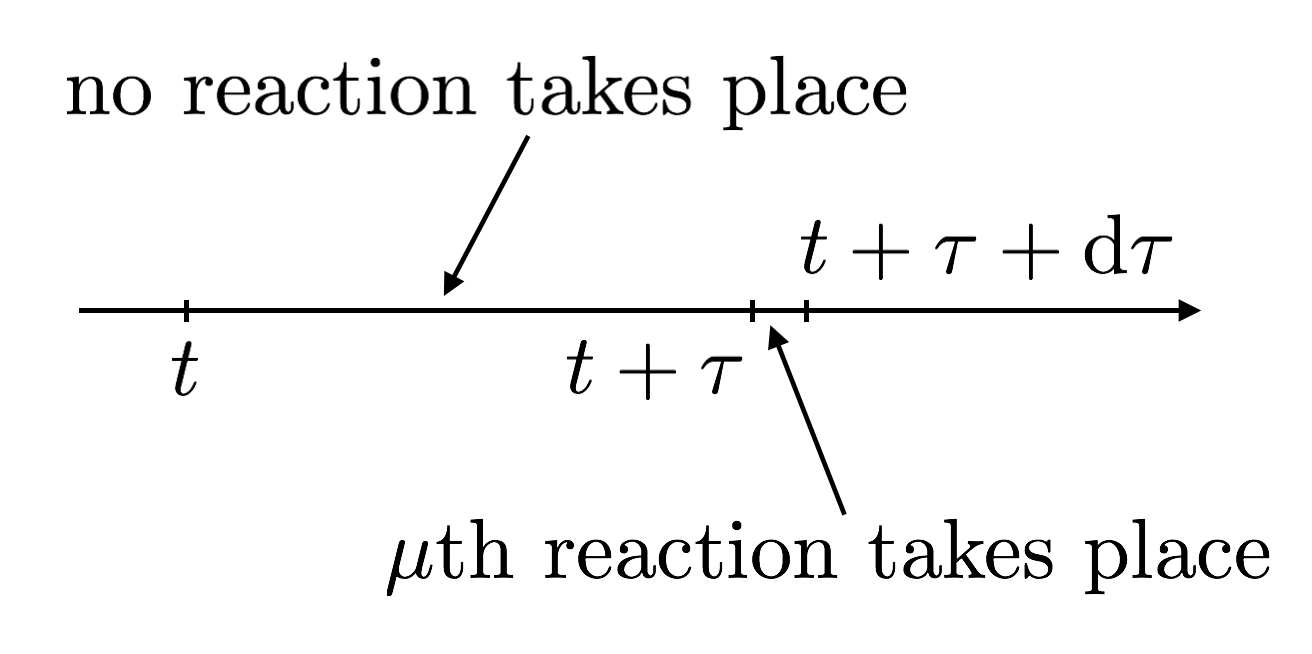
\includegraphics[scale=0.24]{img/reaction_prob.png}
		\caption{explanation of $\rho(\mu,\tau)$ }
		\label{img:reaction_prob}
		\end{wrapfigure}

		Here comes a brief derivation for $\rho(\mu,\tau)$. According to the abovementioned, $\rho(\mu,\tau)$ is a joint probability density of the two events shown in figure \ref{img:reaction_prob}. The probability that $\mu$th reaction takes place in $(t+\tau, t+\tau + \diff \tau]$ simply is, by definition of rate constant, $k_\mu \diff \tau$, and the probability of the other event can be formulated by the following deduction. Firstly divide the interval $(t,t+\tau]$ into $M$ segments whose length of each is a very small number $\varepsilon=\tau / M$. Secondly, consider the probability that $\nu$th reaction does not take place in interval $\varepsilon$, which should be $1-k_\nu\varepsilon$. This implies
		\begin{equation}
			\begin{aligned}
			&p(\text{no reaction takes place in next $\tau$}) \\&=
				\lim_{M\to\infty} \left[ 1-\sum_{\nu}k_\nu\frac{\tau}{M} \right]^{M} 
				=\ee^{-\sum_\nu k_\nu \tau} = \ee^{-K\tau},
			\end{aligned}
			\label{eq:possion}
		\end{equation}
		where \textit{the summation is over all possible reactions at current time} and $K$ denotes the summation for simplicity. So finaly, the reaction probability density is
		\begin{equation}
			\rho(\mu,\tau) = k_\mu \ee^{-K\tau}.
		\end{equation}

		Based on the above knowledge, Gillespie Monte Carlo can be understood without difficulties. The basic idea is to simulate the transition process by continuously generating random variable pairs $(\mu, \tau)$ according the reaction probability density $\rho(\mu,\tau)$. In order to do so, one need calculate the two marginal probabilities of $\rho(\mu,\tau)$ as follows.
		\begin{equation}
			\begin{aligned}
				\rho_0(\tau) &= \sum_\nu k_\nu \rho(\mu,\tau) = K\ee^{-K\tau}\\
				p_0(\mu) &= \int_0^{+\infty}\rho(\mu,\tau)\diff \tau = \frac{k_\mu}{K},
			\end{aligned}
			\label{eq: marginal_distribution}
		\end{equation}
		Thus the transition time $\tau$ is exponentially distributed, and reaction indexes $\mu$ follows a discrete distribution which is proportional to $k_\mu$. As can be seen, the multiplication of the two marginal probabilities recovers the reaction distribution density, which implies the following two events A and B are independent with each other.
		\begin{description}
			\item A: the next transition is the $\mu$th transition.
			\item B: the next transition will take place in time $\tau$.
		\end{description}
		Therefore the pair $(\mu, \tau)$ can be sampled separately according to the following formulas.
		\begin{equation}
			\begin{aligned}
			&\tau = \frac{1}{K}\ln{\frac{1}{r_1}}, \ \ 
			\sum_{\nu=1}^{\mu-1} k_\mu <r_2K \le \sum_{\nu=1}^{\mu} k_\mu\\
			r_1,r_2 \in &(0,1]: \text{uniformly distributed random varibles.}
			\end{aligned}
			\label{eq:sampling}
		\end{equation}
		Then the direct procedure of Gillespie Monte Carlo can be described as follows.
		\begin{enumerate}
			\item Initialization: set $t = 0$ and state $=i$ ($0$ or $1$ in the system described by figure \ref{img:dynamics}).
			\item Sampling: generator random pair $(\mu, \tau)$ by using equation \eqref{eq:sampling}
			\item Update: update current time $t$ by adding $\tau$ and current state by triggering the $\mu$th reaction.
			\item Repeat step $2$ and $3$ for enough times.
			\item Compute the life-span time fractions for states of interest, and regard the fractions as state probabilities.
		\end{enumerate}

		Alternatively, one can use another procedure called "first-reaction" method. In this method, one determines the next reaction and transition time at one time by sampling and comparing the quantities
		\begin{equation}
			\tau_\mu = \frac{1}{k_\mu}\ln{\left(\frac{1}{r}\right)},
			\label{eq:method2}
		\end{equation}
		where $\mu$ varies among all possible transitions with respect to current state, and $r \in (0,1]$ is a uniformly distributed random number. Once these quantities are computed, the shortest $\tau_{\text{shortest}}$ wins and the corresponding transition will be the "first reaction". Then the time will be updated by adding $\tau_{\text{shortest}}$ and the state will be updated according the winning transition.

		Both of these two procedures will be implemented and their results will be compared in the last section, while here I try to show the equivalence of them. The corresponding probability density of the sampling method shown in equation \eqref{eq:method2} is
		\begin{equation}
			\rho_\mu(\tau) = k_\mu \ee^{-k_\mu\tau}.
			\label{eq:partial_tau_prob}
		\end{equation}
		Notice the difference between $\rho_\mu(\tau)$ here and $\rho_0(\tau)$ in equation \eqref{eq: marginal_distribution} is that $\rho_0$ refers to the global transition time while $\rho_\mu$ refers to the transition $\mu$ only. For simplicity, the system shown in figure \ref{img:dynamics} is taken as an example for following derivation without losing any generality. Suppose the system is currently at state $1$, then the two possible transitions are $k_2$ and $k_3$. The corresponding transition time prabability densities of them are denoted as
		\begin{equation}
			\begin{aligned}
			\rho_2(\tau) &= k_2 \ee^{-k_2\tau} \\
			\rho_3(\tau) &= k_3 \ee^{-k_3\tau}.
			\end{aligned}
		\end{equation}
		The meaning of them, taking $\rho_2$ as an example, is that $\rho_2(\tau)\diff \tau$ is the probability that the transition $k_2$ will take place in the next $\diff \tau$, terminating a period with no $k_2$ taking place. 

		The following proof is divided into two parts: the equivalence of the global transition time distribution, and the equivalence of the discrete reaction index distribution.
		To show the first equivalence, one may ask what is the probability that any one transition of the two will take place in the next $\diff \tau$. Explicitly, this is the probability of the following event:
		\begin{quote}
			$k_2$ will take place in the $(t+\tau, t+\tau+\diff \tau]$ AND $k_3$ does not in $(t, t+\tau]$, \\ OR $k_3$ will take place in the $(t+\tau, t+\tau+\diff \tau]$ AND $k_2$ does not in $(t, t+\tau]$.
		\end{quote}
		Then this probability can be written down directly (recall equation \eqref{eq:possion}).
		\begin{equation}
				\rho_2(\tau)\diff\tau \times \ee^{-k_3\tau} + 
				\rho_3(\tau)\diff\tau \times \ee^{-k_2\tau} 
				= (k_2 + k_3) \ee^{-(k_2+k_3)\tau} \diff\tau
		\end{equation}
		Therefore, this recovers the form of $\rho_0$ in equation \eqref{eq: marginal_distribution}. Thus, the global transition time distribution in direct method and "first-reaction" method are the same.
		The second equivalence can be shown by asking, in the regime of "first-reaction" method, what is the probability that the reaction which will firstly take place subsequently is the $\mu$th reaction. Taking $\mu=2$ as an example, this requires us to calculate the probability that $\tau_2<\tau_3$ ($\tau_2$ and $\tau_3$ refer to the quantities in equation \eqref{eq:method2}). This is also a straightforward calculation as follows.
		\begin{equation}
			\begin{aligned}
				p(\tau_2<\tau_3) &= \int_0^{+\infty} \diff \tau_3 \int_0^{\tau_3} \diff \tau_2 \rho(\tau_2,\tau_3) \\
				&=\int_0^{+\infty}\diff\tau_3\int_0^{\tau_3}\diff\tau_2 k_2\ee^{-k_2\tau_2}k_3\ee^{-k_3\tau3}\\
				&=\frac{k_2}{k_2+k_3}.
			\end{aligned}
		\end{equation}
		Here the property of independence is employed so that the joint probability is the multiplication of the two marginal probabilities.
		Again, this recovers the form of $p_0(\mu)$ in equation \eqref{eq: marginal_distribution}. Thus the discrete reaction index distribution also remains the same.

		As a sub-conclusion, one can see the reaction probability density undergoing within the two Gillespie Monte Carlo methods remains the same, which means these two methods are equivalent.
% \newpage
\section{Simulation Result}
	To test Gillespie Monte Carlo algorithm, a simulation for the dynamic system shown in figure \ref{img:dynamics} has been done and the results are displayed in figure \ref{img:direct_result} and \ref{img:first-reaction}.
	\begin{figure}[H]
		\centering
		\begin{subfigure}{0.46\textwidth}
		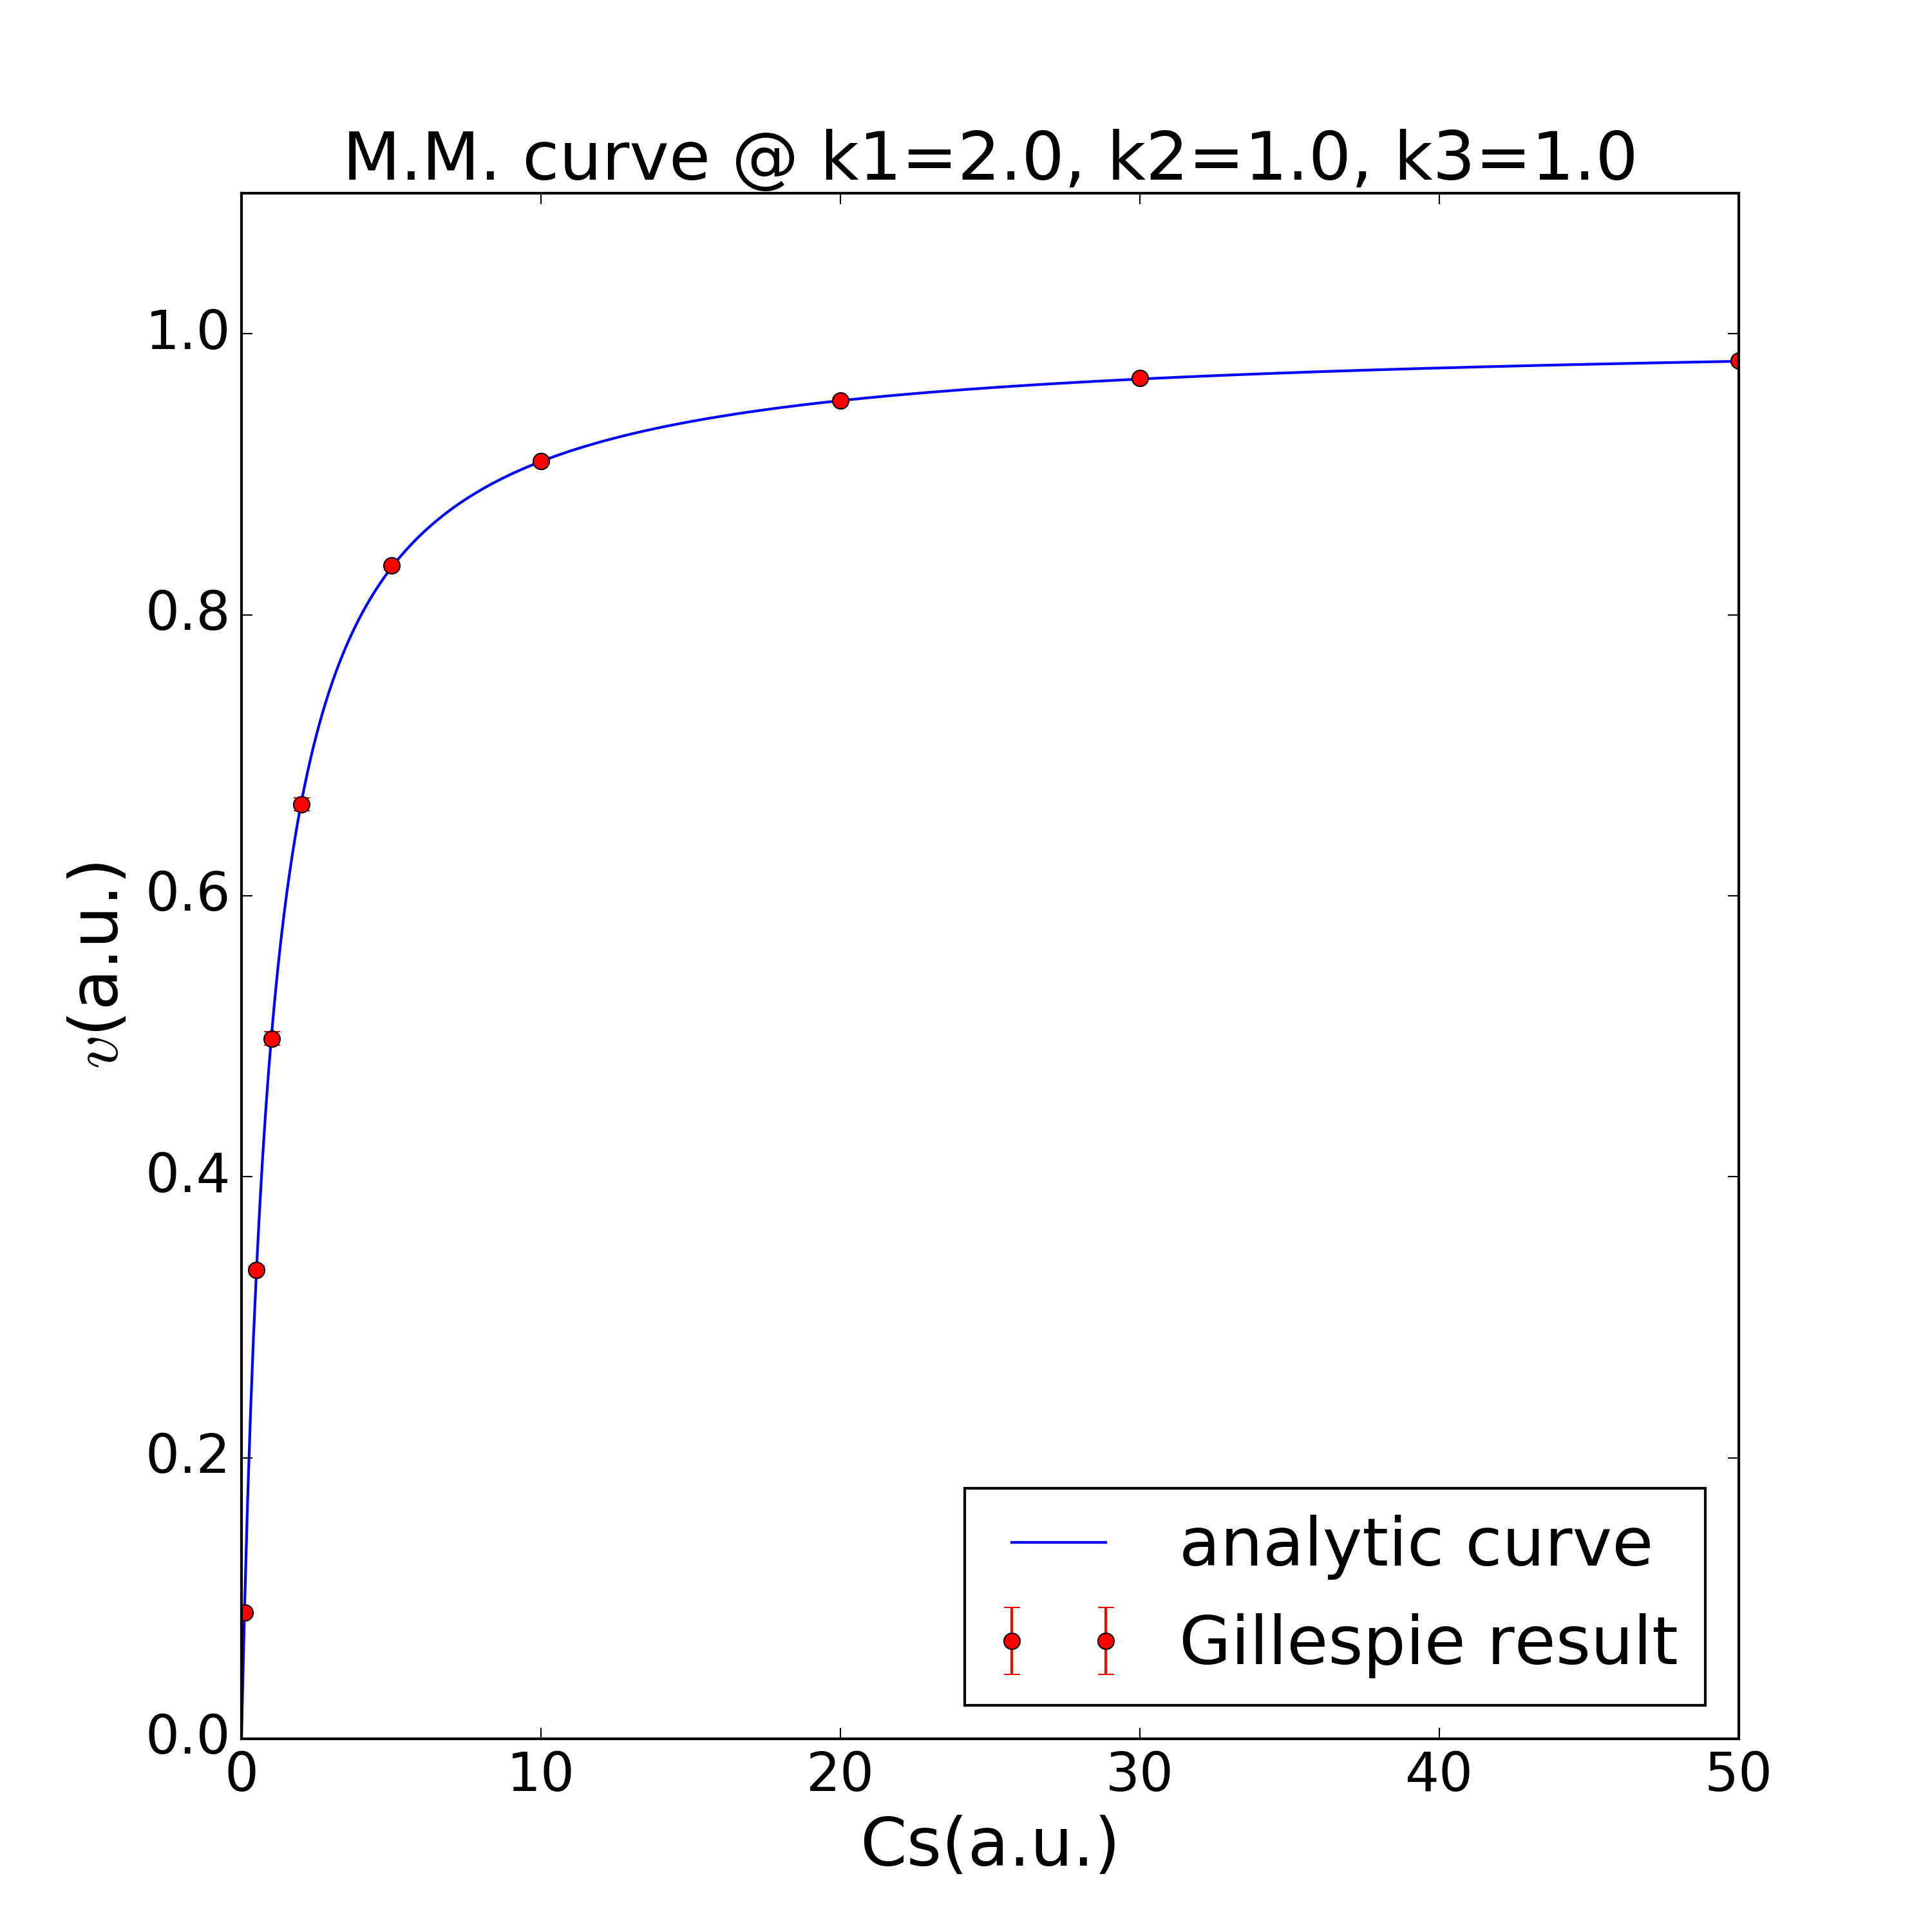
\includegraphics[scale=0.33]{img/MM1.png}
		\caption{M.M. curve}
		\end{subfigure}
		\begin{subfigure}{0.46\textwidth}
		\includegraphics[scale=0.33]{img/state1.png}
		\caption{state-time dependence}
		\end{subfigure}
		\caption{simulation result of direct Gillespie Monte Carlo method}
		\label{img:direct_result}
	\end{figure}

	\begin{figure}[H]
		\centering
		\begin{subfigure}{0.46\textwidth}
		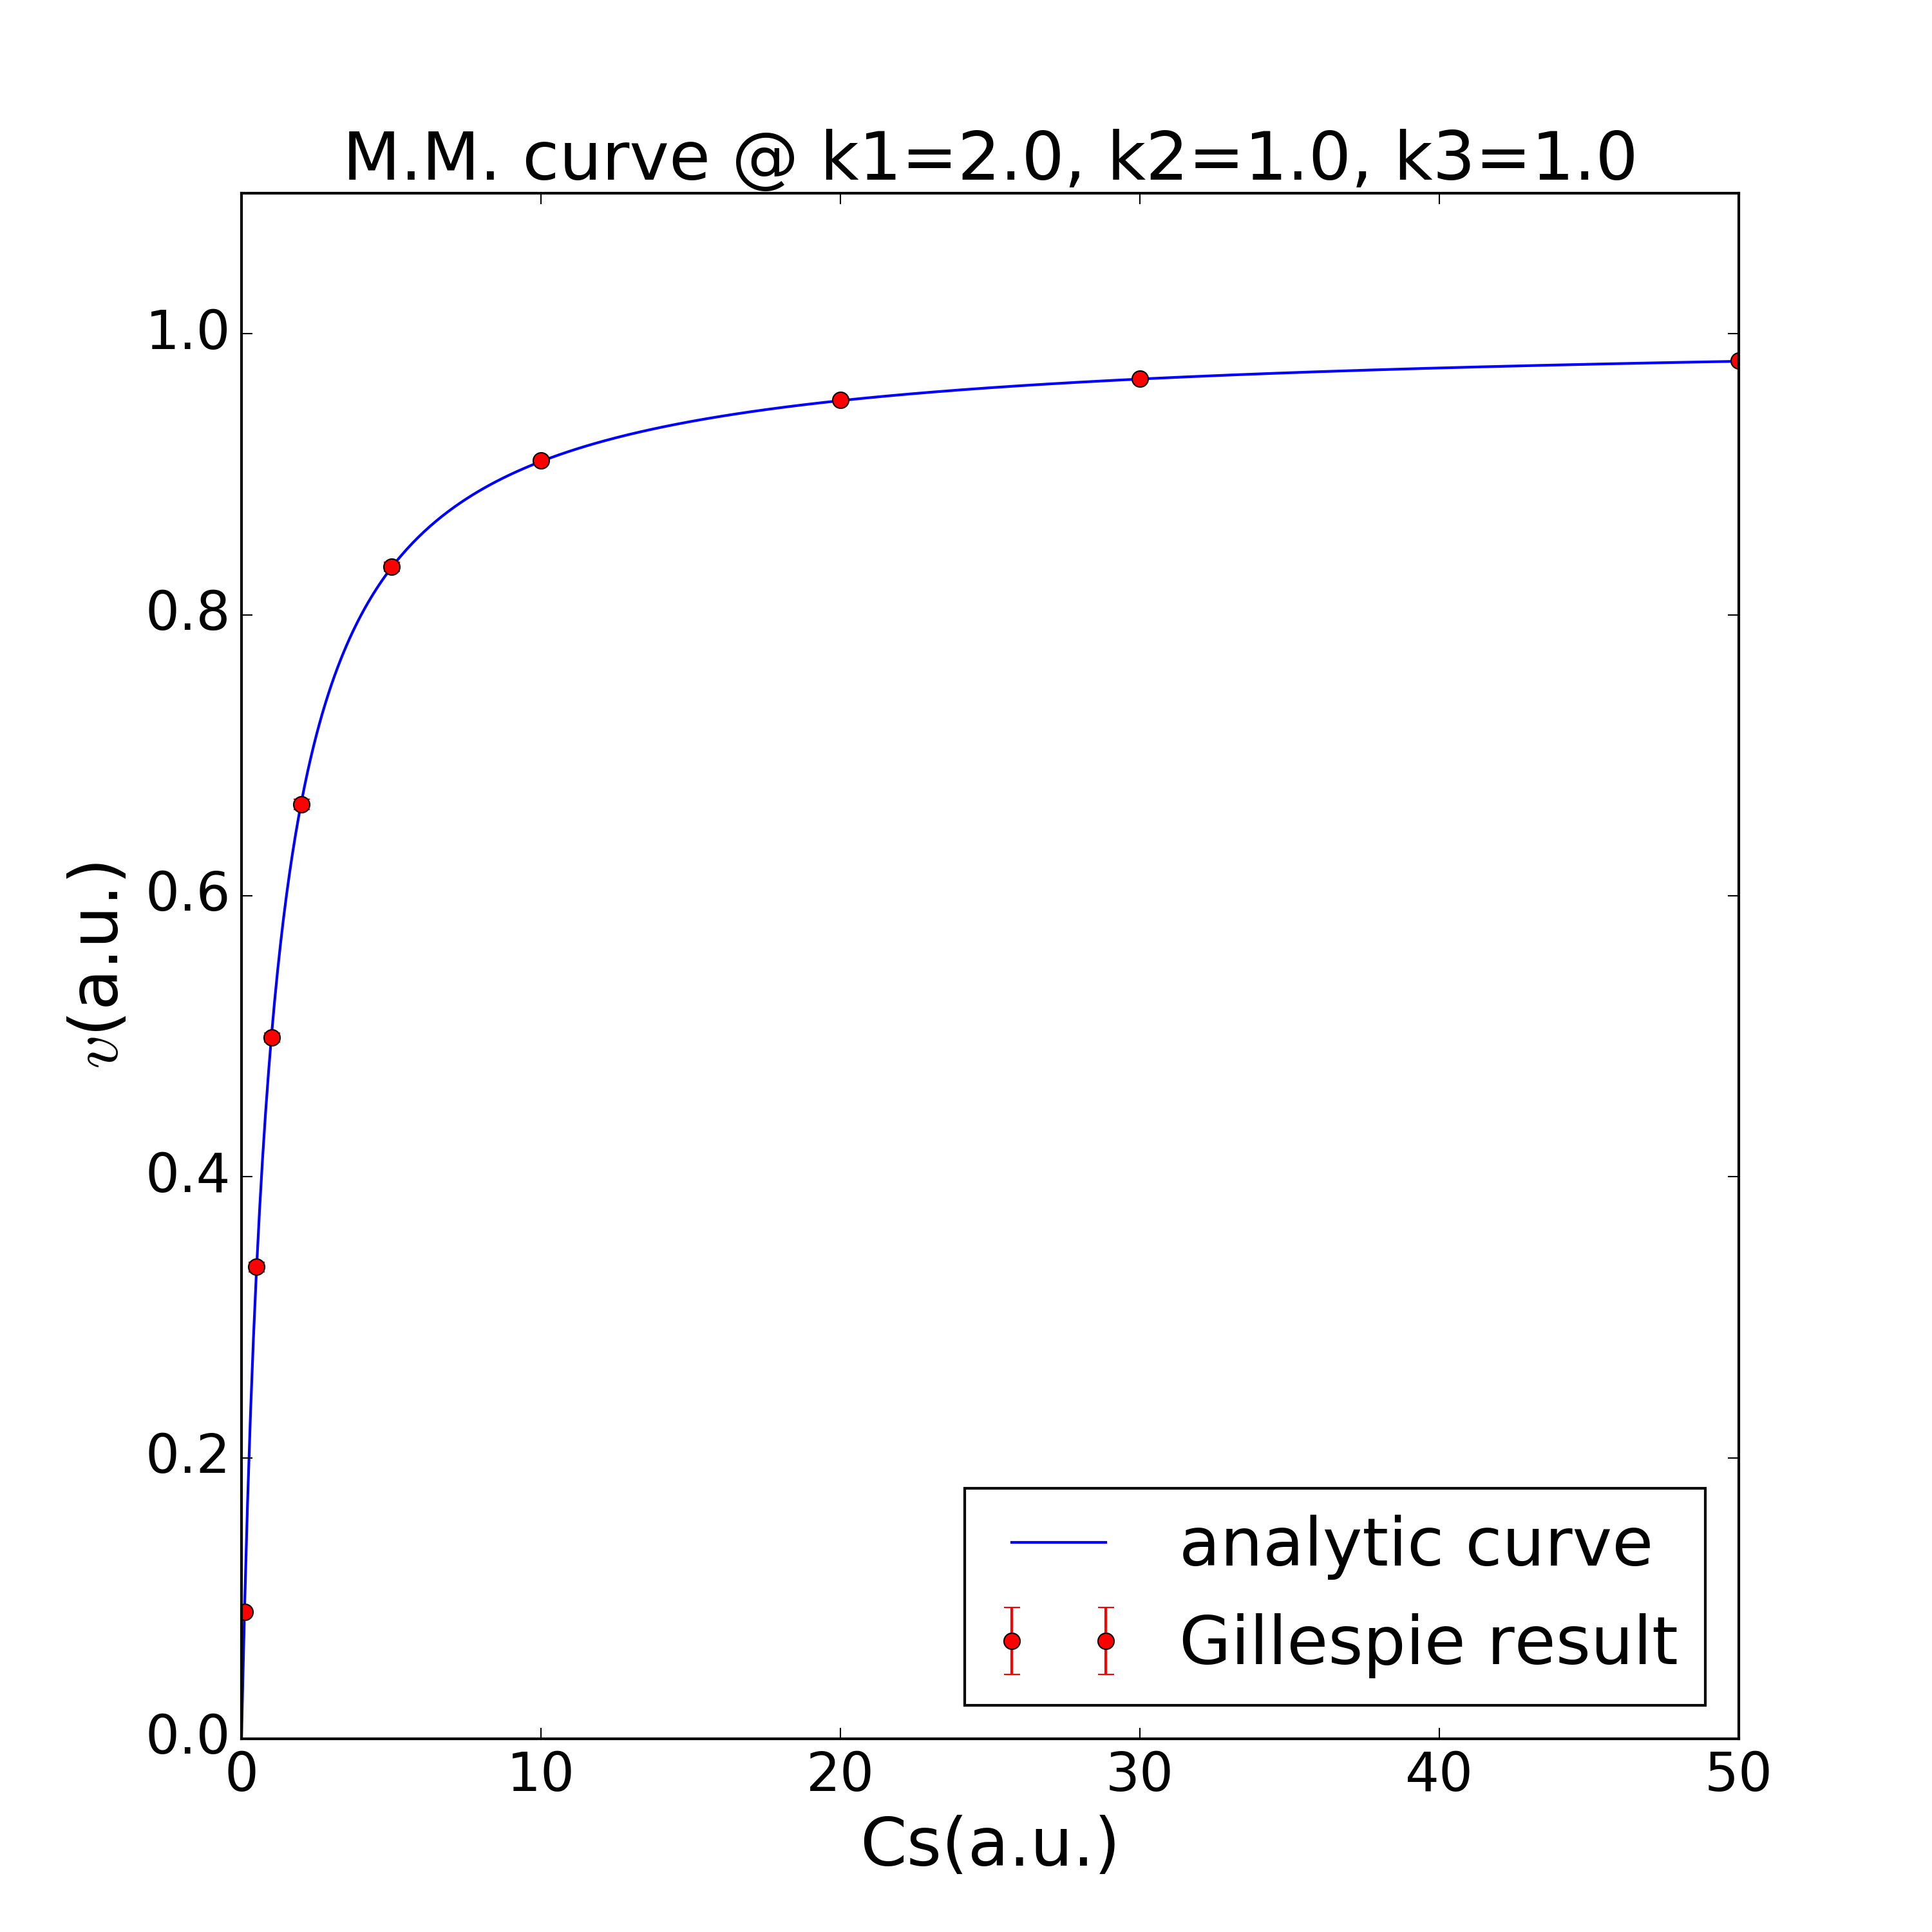
\includegraphics[scale=0.33]{img/MM2.png}
		\caption{M.M. curve}
		\end{subfigure}
		\begin{subfigure}{0.46\textwidth}
		\includegraphics[scale=0.33]{img/state2.png}
		\caption{state-time dependence}
		\end{subfigure}{}
		\caption{simulation result of "first-reaction" Gillespie Monte Carlo method}
		\label{img:first-reaction}
	\end{figure}

	$10,000$ Monte Carlo steps have been run for each substrate concentration point. The errorbars are obtained by computing the standart deviation of each point. As can be seen, both of the two methods function well and a $10,000$-step simulation is enough for the system shown in figure \ref{img:dynamics} due to the very small deviation. The state-time dependence is plotted out as well for four different substrate concentrations. Clearly, as the $C_S$ increases, the average life-span time of state $1$ increases, which is consistent with mechanism described by the chemical equation \eqref{eq:chemical}.

	In conclusion, the equivalence between the direct and "first-reaction" Gillespie methods is shown by both analytic deduction and simulation results. In addition, the simulation results of reaction rate are very consistent with Michaelis Menten equation. For the simple system shown in figure \ref{img:dynamics}, $10,000$ Monte Carlo steps can already give fairly small deviation, while for a more complex system, more might be required to lower the deviation. Because it is easy to program and the error is easy to be controled, Gillespie Monte Carlo algorithm is potentially a powerful method for studying various biochemical systems.





